\hypertarget{main_8cpp}{
\subsection{main.cpp File Reference}
\label{main_8cpp}\index{main.cpp(173)@{main.cpp(173)}}
}
Implementation of a command line program for testing purposes.  


{\tt \#include $<$Magick++.h$>$}\par
{\tt \#include \char`\"{}Recognizer.hpp\char`\"{}}\par
{\tt \#include \char`\"{}DataSet.hpp\char`\"{}}\par
{\tt \#include $<$iostream$>$}\par


Include dependency graph for main.cpp:\nopagebreak
\begin{figure}[H]
\begin{center}
\leavevmode
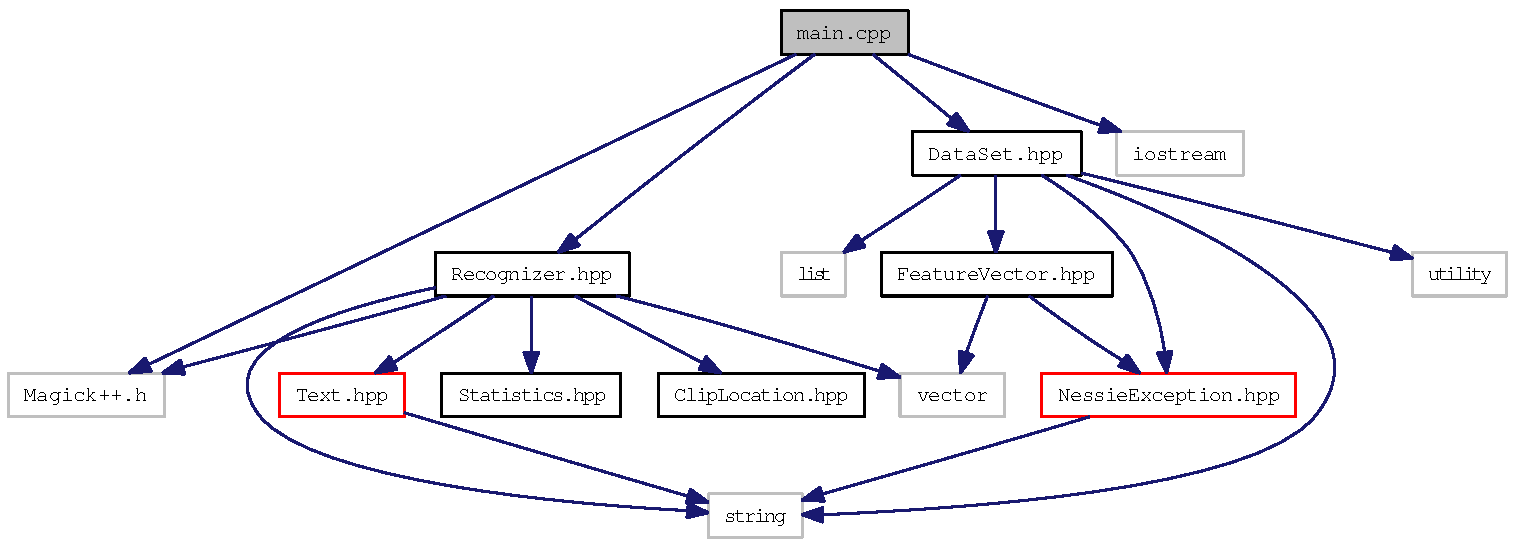
\includegraphics[width=381pt]{main_8cpp__incl}
\end{center}
\end{figure}
\subsubsection*{Functions}
\begin{CompactItemize}
\item 
int \hyperlink{main_8cpp_bf9e6b7e6f15df4b525a2e7705ba3089}{main} (int argc, char const $\ast$argv\mbox{[}$\,$\mbox{]})
\end{CompactItemize}


\subsubsection{Detailed Description}
Implementation of a command line program for testing purposes. 



\subsubsection{Function Documentation}
\hypertarget{main_8cpp_bf9e6b7e6f15df4b525a2e7705ba3089}{
\index{main.cpp@{main.cpp}!main@{main}}
\index{main@{main}!main.cpp@{main.cpp}}
\paragraph[{main}]{\setlength{\rightskip}{0pt plus 5cm}int main (int {\em argc}, \/  char const $\ast$ {\em argv}\mbox{[}$\,$\mbox{]})}\hfill}
\label{main_8cpp_bf9e6b7e6f15df4b525a2e7705ba3089}


\begin{Desc}
\item[\hyperlink{todo__todo000001}{Todo}]Check documentation for pre- and post-conditions.\end{Desc}
\begin{Desc}
\item[\hyperlink{todo__todo000001}{Todo}]Develop the KNN algorithm.\end{Desc}
\begin{Desc}
\item[\hyperlink{todo__todo000001}{Todo}]Develop the \hyperlink{class_classifier}{Classifier} class.\end{Desc}
\begin{Desc}
\item[Parameters:]
\begin{description}
\item[{\em argc}]Number of command line arguments \item[{\em argv}]Command line arguments\end{description}
\end{Desc}
\begin{Desc}
\item[Author:]Eliezer Talón (\href{mailto:elitalon@gmail.com}{\tt elitalon@gmail.com}) \end{Desc}
\begin{Desc}
\item[Date:]2008-10-16 \end{Desc}


Here is the call graph for this function:\nopagebreak
\begin{figure}[H]
\begin{center}
\leavevmode
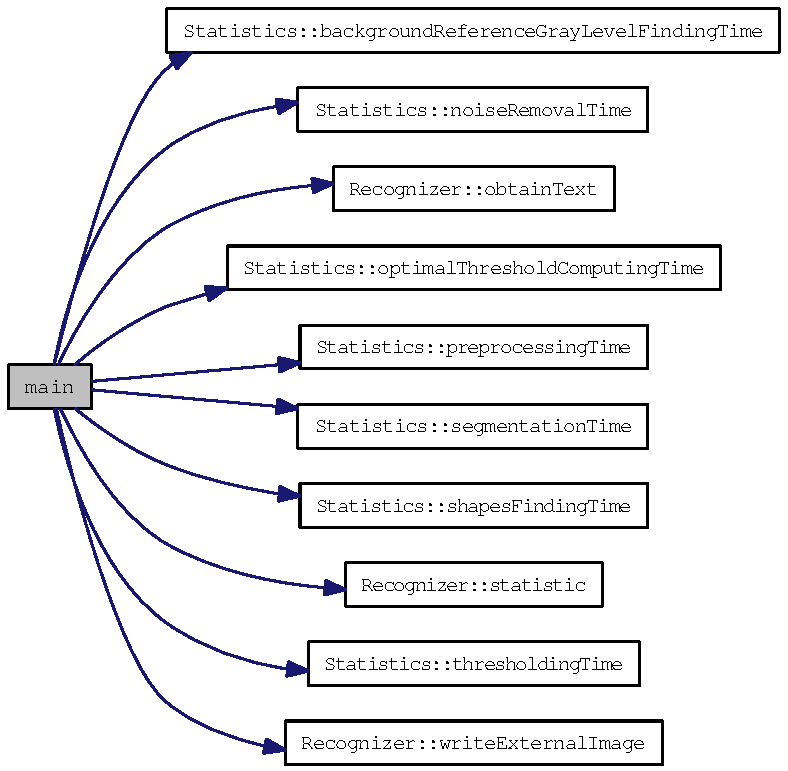
\includegraphics[width=207pt]{main_8cpp_bf9e6b7e6f15df4b525a2e7705ba3089_cgraph}
\end{center}
\end{figure}
